% Compile here: xelatex -jobname=Report_TV3 Report_TV3.tex
\documentclass[conference,a4paper]{IEEEtran}
\usepackage{fontspec}
\setmainfont{Times New Roman}
\setsansfont{Arial}
\setmonofont{Consolas}
\usepackage[english,vietnamese]{babel}
\defaultfontfeatures{Ligatures=TeX}
\usepackage{cite}
\usepackage{amsmath,amssymb,amsfonts,algorithmic,booktabs,graphicx,capt-of,textcomp,xcolor,url}
\usepackage[hidelinks,unicode]{hyperref}
\graphicspath{{figures/}}
\renewcommand{\figurename}{Hình}
\renewcommand{\tablename}{Bảng}
\renewcommand{\refname}{Tài liệu tham khảo}
\makeatletter
\setlength{\@fptop}{0pt}
\setlength{\@fpsep}{12pt}
\setlength{\@fpbot}{0pt plus 1fil}
\setlength{\@dblfptop}{0pt}
\setlength{\@dblfpsep}{12pt}
\setlength{\@dblfpbot}{0pt plus 1fil}
\makeatother
\begin{document}
\selectlanguage{vietnamese}
\raggedbottom
\title{Khai thác tập mục phổ biến từ ảnh Fashion-MNIST}
\author{\IEEEauthorblockN{Nguyễn Võ Tấn Duy}
\IEEEauthorblockA{Thành viên 3 --- Đồ án môn Khai thác dữ liệu và ứng dụng\\
Trường Đại học Khoa học Tự nhiên, ĐHQG-HCM}}
\maketitle

\begin{abstract}
Báo cáo chuyển 70.000 ảnh Fashion-MNIST thành giao dịch túi từ thị giác
nhị phân và khai thác tập mục phổ biến bằng hai backend Eclat. K-means
với 32 cụm hội tụ sau 220 vòng trong giới hạn 400 vòng; hai backend
khớp kết quả tại cả sáu ngưỡng, với 6.185 tập mục ở minsup 5\%. Các mẫu
được đối chiếu với ảnh và phân tích theo lớp. Thời gian một lượt ở
ngưỡng 5\% là 20,94 giây với Set và 8,73 giây với BitVector; do không
có warm-up hay đo lặp, số liệu này chỉ có giá trị tham khảo. Vì cả ảnh
huấn luyện và kiểm thử được dùng để học từ điển và khai thác, kết quả
hỗ trợ phân tích mô tả, không phải đánh giá phân loại độc lập.
\end{abstract}

\begin{IEEEkeywords}
Fashion-MNIST, túi từ thị giác nhị phân, Eclat, tập mục phổ biến.
\end{IEEEkeywords}

\setcounter{section}{2}
\section{Khai thác mẫu trực quan phổ biến trên Fashion-MNIST}

\subsection{Bài toán và tập dữ liệu}

Trong dữ liệu giao dịch, khai thác tập mục phổ biến giúp tìm những mục thường đi cùng nhau. Để áp dụng Eclat cho ảnh, nhóm biểu diễn mỗi vùng ảnh nhỏ bằng một từ thị giác (\textit{visual word}) và xem tập các từ xuất hiện trong một ảnh là một giao dịch. Mỗi tập mục phổ biến tìm được vì thế tương ứng với một tổ hợp từ thị giác thường cùng xuất hiện trong ảnh.

Tập dữ liệu \href{https://github.com/zalandoresearch/fashion-mnist}{Fashion-MNIST}~\cite{Xiao2017} gồm 70.000 ảnh xám kích thước $28 \times 28$ pixel, chia đều cho 10 lớp sản phẩm thời trang. Bảng~\ref{tab:fashionmnist_distribution} cho biết số ảnh của từng lớp trong hai tập gốc. Nhóm dùng cả hai tập để khai thác mẫu, đối chiếu một số mẫu với ảnh gốc và khảo sát mức độ phổ biến của chúng trong từng lớp.

Các ảnh có cùng kích thước nên có thể chia theo một lưới chung và đối chiếu các vùng được gán mã với ảnh gốc. Mỗi lớp có cùng số ảnh, giúp việc so sánh tỷ lệ xuất hiện của mẫu giữa các lớp dễ diễn giải.

\begin{table}[!t]
    \centering
    \caption{Số ảnh theo lớp trong Fashion-MNIST}
    \label{tab:fashionmnist_distribution}
    \footnotesize
    \setlength{\tabcolsep}{3pt}
    \begin{tabular}{@{}c l r r r@{}}
        \hline
        \textbf{Mã} & \textbf{Lớp} & \textbf{Huấn luyện} &
        \textbf{Kiểm thử} & \textbf{Tổng} \\
        \hline
        0 & T-shirt/top  & 6.000 & 1.000 & 7.000 \\
        1 & Trouser      & 6.000 & 1.000 & 7.000 \\
        2 & Pullover     & 6.000 & 1.000 & 7.000 \\
        3 & Dress        & 6.000 & 1.000 & 7.000 \\
        4 & Coat         & 6.000 & 1.000 & 7.000 \\
        5 & Sandal       & 6.000 & 1.000 & 7.000 \\
        6 & Shirt        & 6.000 & 1.000 & 7.000 \\
        7 & Sneaker      & 6.000 & 1.000 & 7.000 \\
        8 & Bag          & 6.000 & 1.000 & 7.000 \\
        9 & Ankle boot   & 6.000 & 1.000 & 7.000 \\
        \hline
          & \textbf{Tổng} & \textbf{60.000} & \textbf{10.000} & \textbf{70.000} \\
        \hline
    \end{tabular}
\end{table}

\subsection{Xây dựng cơ sở dữ liệu giao dịch từ ảnh}

Hình~\ref{fig:fashion_tc_pipeline} tóm tắt các bước chuyển ảnh Fashion-MNIST thành cơ sở dữ liệu giao dịch bằng BoVW nhị phân.

\begin{figure*}[!t]
    \centering
    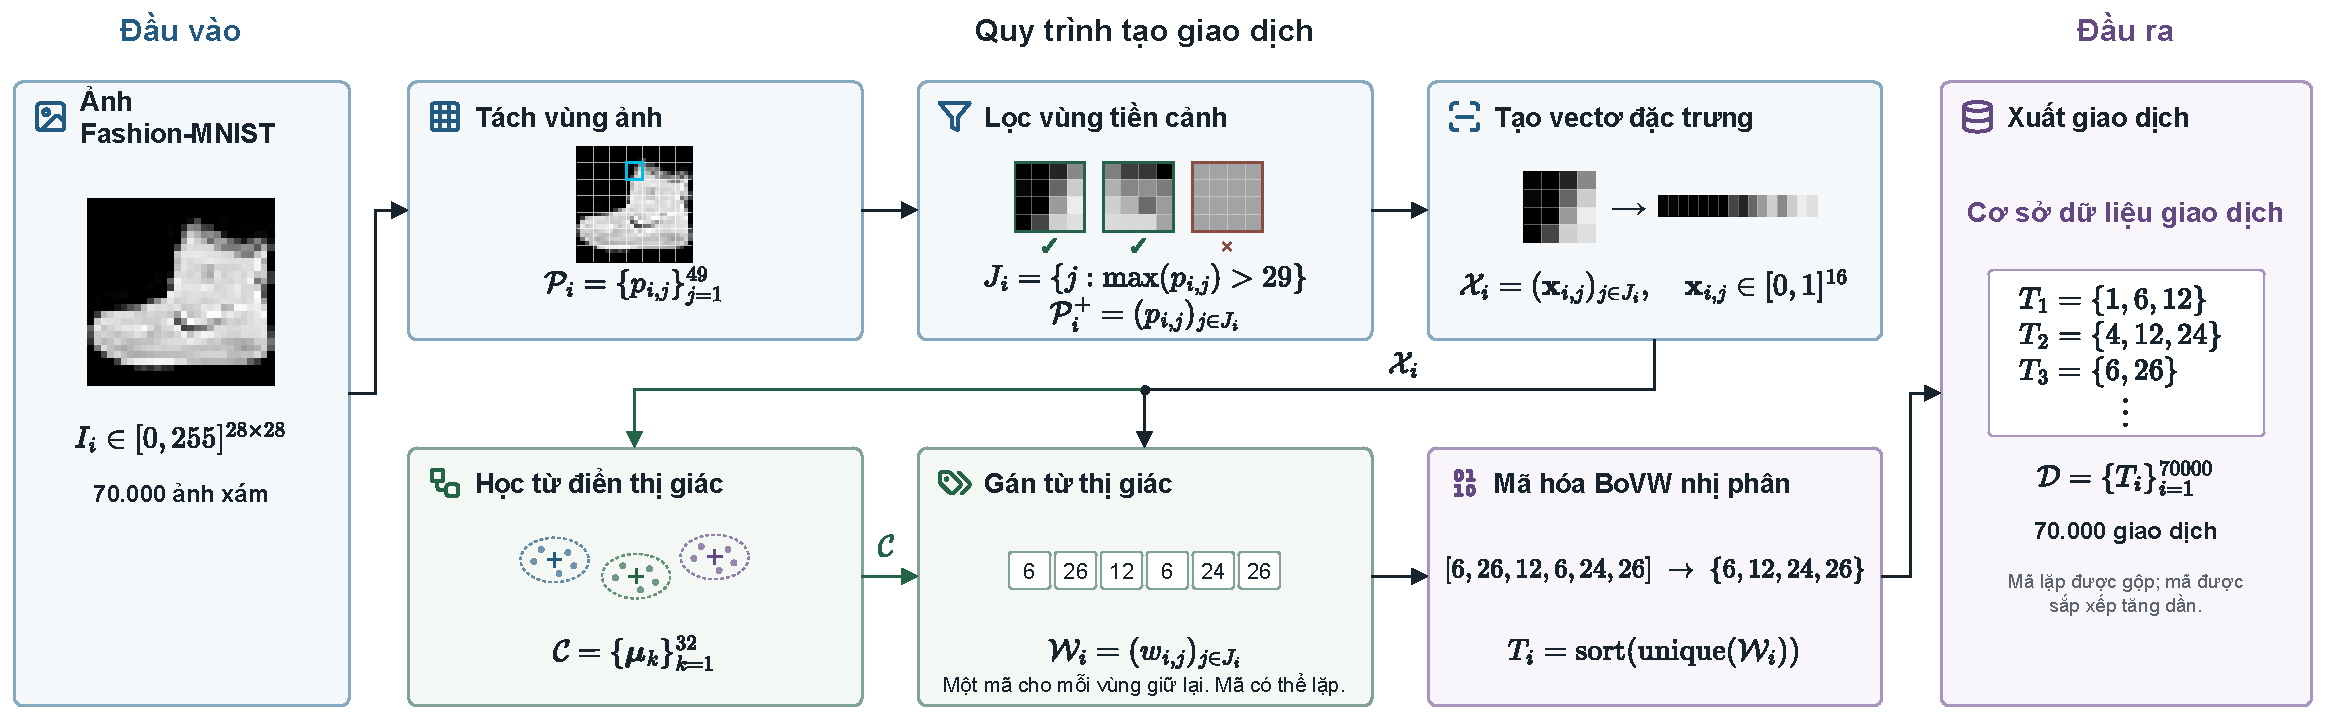
\includegraphics[width=\textwidth]{figures/diagram/TC_pipeline.pdf}
    \caption{Quy trình tạo giao dịch từ ảnh Fashion-MNIST. Nhóm học một từ điển chung từ các vùng giữ lại trên toàn bộ 70.000 ảnh rồi dùng từ điển đó để gán mã cho từng vùng. Các mã và giao dịch trong hình dùng để minh họa.}
    \label{fig:fashion_tc_pipeline}
\end{figure*}

Nhóm tạo giao dịch theo phương pháp túi từ thị giác (\textit{Bag of Visual Words}, BoVW)~\cite{Sivic03}. Mỗi ảnh được chia thành 49 vùng $4 \times 4$ pixel không chồng lấn. Trong bước khám phá dữ liệu, khi cả hai lưới đều loại khoảng 39,3\% số vùng, lưới $4\times4$ chỉ mất 5,92\% tổng độ lớn gradient, so với 14,00\% ở lưới $7\times7$. Kết quả này là cơ sở để chọn lưới $4\times4$ cho bước lọc nền.

Để lọc nền, nhóm chọn ngưỡng 29, tức phân vị 10\% của các điểm ảnh có giá trị lớn hơn 0 (Q10+). Quy tắc giữ vùng có ít nhất một điểm ảnh vượt ngưỡng loại 37,50\% số vùng và làm mất 4,41\% tổng độ lớn gradient. Mọi ảnh đều còn vùng sau khi lọc, với tổng cộng 2.143.746 trên 3.430.000 vùng được giữ. Trong mỗi vùng giữ lại, nhóm đọc 16 giá trị mức xám theo thứ tự cột rồi chia cho 255 để tạo vectơ trong $[0,1]^{16}$.

Nhóm dùng K-means~\cite{Hartigan1979} để phân cụm 2.143.746 vectơ thu được từ các vùng được giữ lại. Codebook thị giác gồm 32 tâm cụm, $\mathcal{C}=\{\boldsymbol{\mu}_k\}_{k=1}^{32}$. Với descriptor $\mathbf{x}_{i,j}$ của vùng được giữ lại, mã gán là $w_{i,j}=\arg\min_{k\in\{1,\ldots,32\}}\|\mathbf{x}_{i,j}-\boldsymbol{\mu}_k\|_2^2$. Bảng~\ref{tab:kmeans_configuration} ghi cấu hình K-means dùng trong thí nghiệm.

\begin{table}[!t]
    \centering
        \caption{Cấu hình K-means trong thí nghiệm Fashion-MNIST}
    \label{tab:kmeans_configuration}
    \footnotesize
    \setlength{\tabcolsep}{3pt}
    \begin{tabular}{@{}p{0.40\columnwidth} p{0.55\columnwidth}@{}}
        \hline
        \textbf{Tham số} & \textbf{Giá trị} \\
        \hline
        Phương pháp & K-means toàn bộ, khởi tạo K-means++ \\
        Dữ liệu phân cụm & 2.143.746 descriptor từ 70.000 ảnh \\
        Vectơ đặc trưng & 16 giá trị pixel xám đã chuẩn hóa \\
        Số cụm ($K$), seed & 32, 123 \\
        Giới hạn lặp, dung sai & 400, $10^{-4}$ \\
        \hline
    \end{tabular}
\end{table}

Ở bước cuối, với ảnh $I_i$, gọi $J_i$ là tập chỉ số các vùng được giữ lại và $\mathcal{W}_i=(w_{i,j})_{j\in J_i}$ là dãy mã được gán cho các vùng đó. BoVW nhị phân tạo giao dịch $T_i=\operatorname{sort}(\operatorname{unique}(\mathcal{W}_i))$: mỗi mã chỉ xuất hiện một lần và các mã được sắp xếp tăng dần. Tọa độ vùng được lưu riêng để truy vết, không đưa vào $T_i$. Bộ giao dịch hiện tại có 70.000 ảnh, không có giao dịch rỗng, tổng cộng 856.373 lượt xuất hiện của 32 mã. Độ dài trung bình là 12,2339 mã, trung vị 12; chi tiết phân bố được trình bày trong Phụ lục~\ref{app:fashion_configuration}.

\subsection{Thiết kế thực nghiệm khai thác}

Eclat tổ chức dữ liệu theo chiều dọc~\cite{Zaki2000}. Với mỗi mã thị giác, thuật toán lưu danh sách số thứ tự các giao dịch có chứa mã đó. Với tập mã $X$, thuật toán lấy phần giao giữa các danh sách tương ứng; số giao dịch còn lại là số ảnh chứa đồng thời mọi mã trong $X$. Nhóm so sánh hai cách lưu các danh sách này trên cùng bộ giao dịch BoVW nhị phân: Set lưu các số thứ tự hiện diện, còn BitVector biểu diễn chúng bằng các bit và lấy phần giao bằng phép AND.

Thực nghiệm dùng sáu ngưỡng hỗ trợ tối thiểu (\textit{minsup}), từ 80\% đến 5\%. Bảng~\ref{tab:fim_minsup} quy đổi mỗi ngưỡng thành số giao dịch cần có trên tổng số 70.000 giao dịch.

\begin{table}[!t]
    \centering
    \caption{Các ngưỡng hỗ trợ tối thiểu dùng trong thực nghiệm}
    \label{tab:fim_minsup}
    \begin{tabular}{c r}
        \hline
        \textbf{Ngưỡng (\%)} & \textbf{Số giao dịch tối thiểu} \\
        \hline
        80 & 56.000 \\
        60 & 42.000 \\
        40 & 28.000 \\
        20 & 14.000 \\
        10 &  7.000 \\
         5 &  3.500 \\
        \hline
    \end{tabular}
\end{table}

Nhóm khảo sát sáu ngưỡng để theo dõi số lượng, độ dài của các tập mục và chi phí khai thác. Ngưỡng 80\% xét các mẫu có mặt trong phần lớn ảnh. Ngưỡng 5\% mở rộng phạm vi phân tích theo lớp và vẫn yêu cầu mỗi mẫu xuất hiện trong ít nhất 3.500 ảnh.

Ở mỗi ngưỡng, nhóm đối chiếu toàn bộ tập mục và số giao dịch hỗ trợ của hai cách biểu diễn. Phần thực nghiệm cũng đo thời gian chạy trong tiến trình Julia riêng cho từng cách cài đặt và ngưỡng. Mỗi cấu hình chỉ được đo một lượt, không có lượt làm nóng hay đo lặp; vì vậy các số đo thời gian chỉ có giá trị tham khảo và được diễn giải thận trọng trong Phụ lục~\ref{app:fashion_eclat}.

\subsection{Kết quả K-means và khai thác tập mục phổ biến}
\label{subsec:fashion_fim_results}

K-means hội tụ theo tiêu chí của thư viện sau 220 vòng trong giới hạn 400 vòng. Độ méo bình phương trung bình là 0,351112; cả 32 cụm đều có phần tử, cụm lớn nhất chứa 11,75\% descriptor và entropy chuẩn hóa đạt 0,9265. Thời gian fit ghi nhận là 137,47 giây.

Set và BitVector được chạy trên cùng 70.000 giao dịch. Hai backend trả về cùng tập mục và cùng số hỗ trợ ở cả sáu ngưỡng; kiểm tra bao hàm cũng xác nhận các tập ở ngưỡng cao hơn vẫn có mặt khi hạ ngưỡng. Bảng~\ref{tab:eclat_backend_comparison} tổng hợp kết quả thí nghiệm.

\begin{table}[!t]
    \centering
    \caption{Số tập mục phổ biến và đối chiếu hai backend}
    \label{tab:eclat_backend_comparison}
    \footnotesize
    \setlength{\tabcolsep}{4pt}
    \begin{tabular}{@{}c r r r c@{}}
        \toprule
        \textbf{Ngưỡng} & \textbf{Số hỗ trợ tối thiểu} &
        \textbf{Set} & \textbf{BitVector} & \textbf{Giống nhau} \\
        \midrule
        80\% & 56.000 & 0 & 0 & PASS \\
        60\% & 42.000 & 1 & 1 & PASS \\
        40\% & 28.000 & 11 & 11 & PASS \\
        20\% & 14.000 & 145 & 145 & PASS \\
        10\% & 7.000 & 1.098 & 1.098 & PASS \\
         5\% & 3.500 & 6.185 & 6.185 & PASS \\
        \bottomrule
    \end{tabular}
\end{table}

Ở ngưỡng 5\%, 6.185 tập mục có độ hỗ trợ ít nhất 3.500 ảnh. Trong đó, 32 tập có một mã, 482 tập có hai mã, 2.468 tập có ba mã, 2.681 tập có bốn mã, 508 tập có năm mã và 14 tập có sáu mã. Các tập ba và bốn mã chiếm 83,22\% kết quả ở ngưỡng này. Trong phép đo một lượt, TID-set mất 20,94 giây và BitVector mất 8,73 giây ở ngưỡng 5\%, tương ứng tỷ số 2,40 lần. Ở ngưỡng 40\%, BitVector chậm hơn nhẹ (5,38 giây so với 5,26 giây của TID-set), nên kết quả này không cho thấy BitVector luôn nhanh hơn. Hình~\ref{fig:eclat_performance} minh họa thời gian chạy theo ngưỡng; bảng số liệu cùng giới hạn diễn giải được nêu trong Phụ lục~\ref{app:fashion_eclat}.

\begin{figure}[!t]
    \centering
    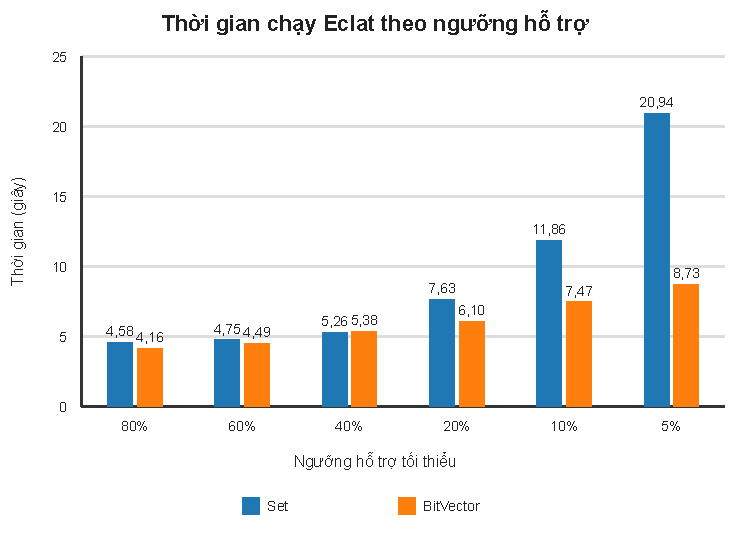
\includegraphics[width=\columnwidth]{figures/notebook3/eclat_performance.pdf}
    \caption{Thời gian chạy một lượt của TID-set và BitVector theo ngưỡng hỗ trợ.}
    \label{fig:eclat_performance}
\end{figure}

\subsection{Truy vết một mẫu từ thị giác}
\label{subsec:visual_pattern_interpretation}

Để minh họa kết quả, nhóm chọn trong các tập mục nhiều mã mẫu có độ hỗ trợ cao nhất ở ngưỡng 5\%, phá hòa theo thứ tự từ điển. Mẫu được chọn là $\{6,12\}$, xuất hiện trong 29.223 ảnh, tương ứng 41,747\% toàn bộ giao dịch. Số hỗ trợ được đếm lại trực tiếp và khớp với Eclat.

Hình~\ref{fig:current_pattern_6_12} đặt ảnh minh họa cạnh hai vùng ảnh được gán mã 6 và 12 cùng tâm cụm tương ứng. Trong ảnh này, hai vùng lần lượt nằm ở hàng 5, cột 6 và hàng 6, cột 6 của lưới. Đây là vị trí quan sát được ở một ảnh; BoVW nhị phân chỉ ghi nhận sự hiện diện của hai mã và không ràng buộc chúng phải xuất hiện ở vị trí cố định.

\begin{figure*}[!t]
    \centering
    \begin{tabular}{ccccc}
        
\includegraphics[width=0.17\textwidth]{figures/current_pattern/supporting_image.png} &
        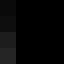
\includegraphics[width=0.17\textwidth]{figures/current_pattern/word_6_actual.png} &
        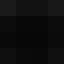
\includegraphics[width=0.17\textwidth]{figures/current_pattern/word_6_centroid.png} &
        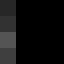
\includegraphics[width=0.17\textwidth]{figures/current_pattern/word_12_actual.png} &
        
\includegraphics[width=0.17\textwidth]{figures/current_pattern/word_12_centroid.png} \\
        Ảnh minh họa & Vùng mã 6 & Tâm mã 6 & Vùng mã 12 & Tâm mã 12
    \end{tabular}
    \caption{Ảnh và các vùng được truy vết cho mẫu $\{6,12\}$. Hai tâm cụm là descriptor mức xám $4\times4$; hình ảnh minh họa một trường hợp gán mã, không đại diện cho mọi ảnh hỗ trợ.}
    \label{fig:current_pattern_6_12}
\end{figure*}

\subsection{Phân bố mẫu theo lớp}
\label{subsec:fim_class_applications}

Sau khi chọn mẫu bằng độ hỗ trợ trên toàn bộ giao dịch, nhóm dùng nhãn lớp trong metadata để mô tả phân bố của mẫu. Với tập mục $X$ và lớp $c$, hệ số làm giàu được tính như sau:
\begin{equation}
    E(X,c)=\frac{P(X\mid c)}{P(X)}.
    \label{eq:fim_F_class_enrichment}
\end{equation}
Giá trị lớn hơn 1 cho biết tỷ lệ ảnh chứa mẫu trong lớp cao hơn tỷ lệ trên toàn bộ ảnh. Bảng~\ref{tab:pattern_class_distribution} ghi kết quả cho mẫu $\{6,12\}$.

\begin{table}[!t]
    \centering
    \caption{Phân bố mẫu $\{6,12\}$ theo lớp}
    \label{tab:pattern_class_distribution}
    \scriptsize
    \setlength{\tabcolsep}{2pt}
    \begin{tabular}{@{}l r r r@{}}
        \toprule
        \textbf{Lớp} & \textbf{Ảnh chứa mẫu} & \textbf{Tỷ lệ trong lớp} & \textbf{Hệ số làm giàu} \\
        \midrule
        T-shirt/top & 4.354 & 62,20\% & 1,490 \\
        Trouser & 1.263 & 18,04\% & 0,432 \\
        Pullover & 3.528 & 50,40\% & 1,207 \\
        Dress & 3.144 & 44,91\% & 1,076 \\
        Coat & 3.593 & 51,33\% & 1,230 \\
        Sandal & 3.360 & 48,00\% & 1,150 \\
        Shirt & 4.323 & 61,76\% & 1,479 \\
        Sneaker & 1.383 & 19,76\% & 0,473 \\
        Bag & 2.927 & 41,81\% & 1,002 \\
        Ankle boot & 1.348 & 19,26\% & 0,461 \\
        \bottomrule
    \end{tabular}
\end{table}

Mẫu xuất hiện ở cả mười lớp. Tỷ lệ cao nhất là 62,20\% ở T-shirt/top (hệ số 1,490); thấp nhất là 18,04\% ở Trouser (hệ số 0,432). Như vậy, mẫu phổ biến rộng trong dữ liệu nhưng mức độ phổ biến khác nhau giữa các lớp; riêng hệ số cao nhất là 1,49, không cho thấy mẫu chỉ thuộc về một lớp.

Phân tích này dùng nhãn sau khi khai thác để mô tả nhóm ảnh chứa mẫu, không dùng nhãn để tạo giao dịch. Tuy nhiên, từ điển và các tập mục của lượt hiện tại được xây dựng trên cả 60.000 ảnh huấn luyện và 10.000 ảnh kiểm thử. Vì vậy, phân bố trên không phải đánh giá độc lập trên tập kiểm thử và không chứng minh khả năng phân loại.

\subsection{Mức độ làm giàu theo ngưỡng hỗ trợ}

Với mỗi tập mục $X$, đặt $E_{\max}(X)=\max_c E(X,c)$, tức hệ số làm giàu lớn nhất trong mười lớp. Bảng~\ref{tab:fashion_enrichment_thresholds} cho thấy cả trung vị $E_{\max}$ lẫn tỷ lệ tập mục có $E_{\max}\geq2$ tăng khi hạ ngưỡng hỗ trợ. Tại 5\%, 4.180 trong 6.185 tập mục (67,58\%) có tỷ lệ xuất hiện trong ít nhất một lớp cao ít nhất gấp đôi tỷ lệ chung; ở các ngưỡng 40\% trở lên, không có tập nào đạt mức này.

\begin{table}[!t]
    \centering
    \caption{Hệ số làm giàu lớn nhất theo ngưỡng hỗ trợ}
    \label{tab:fashion_enrichment_thresholds}
    \scriptsize
    \setlength{\tabcolsep}{3pt}
    \begin{tabular}{@{}c r r r r@{}}
        \toprule
        \textbf{Ngưỡng} & \textbf{Số tập mục} & \textbf{Trung vị $E_{\max}$} &
        \textbf{$E_{\max}\geq2$} & \textbf{Tỷ lệ} \\
        \midrule
        80\% & 0 & -- & 0 & -- \\
        60\% & 1 & 1,294 & 0 & 0\% \\
        40\% & 11 & 1,490 & 0 & 0\% \\
        20\% & 145 & 1,735 & 26 & 17,93\% \\
        10\% & 1.098 & 1,998 & 543 & 49,45\% \\
         5\% & 6.185 & 2,225 & 4.180 & 67,58\% \\
        \bottomrule
    \end{tabular}
\end{table}

Hình~\ref{fig:fashion_enrichment_summary} liên hệ kết quả theo ngưỡng với số lượng tập được làm giàu ít nhất gấp đôi trong từng lớp. Các số đếm theo lớp không loại trừ nhau: một tập mục có thể đạt $E(X,c)\geq2$ ở nhiều lớp. $E_{\max}$ cũng là giá trị lớn nhất sau khi xét mười lớp, nên phần tăng này chỉ mô tả các liên hệ trong dữ liệu đã khai thác; không phải phép kiểm định hay bằng chứng rằng các tập mục phân loại được nhãn.

\begin{figure*}[!t]
    \centering
    \begin{minipage}[t]{0.48\textwidth}
        \centering
        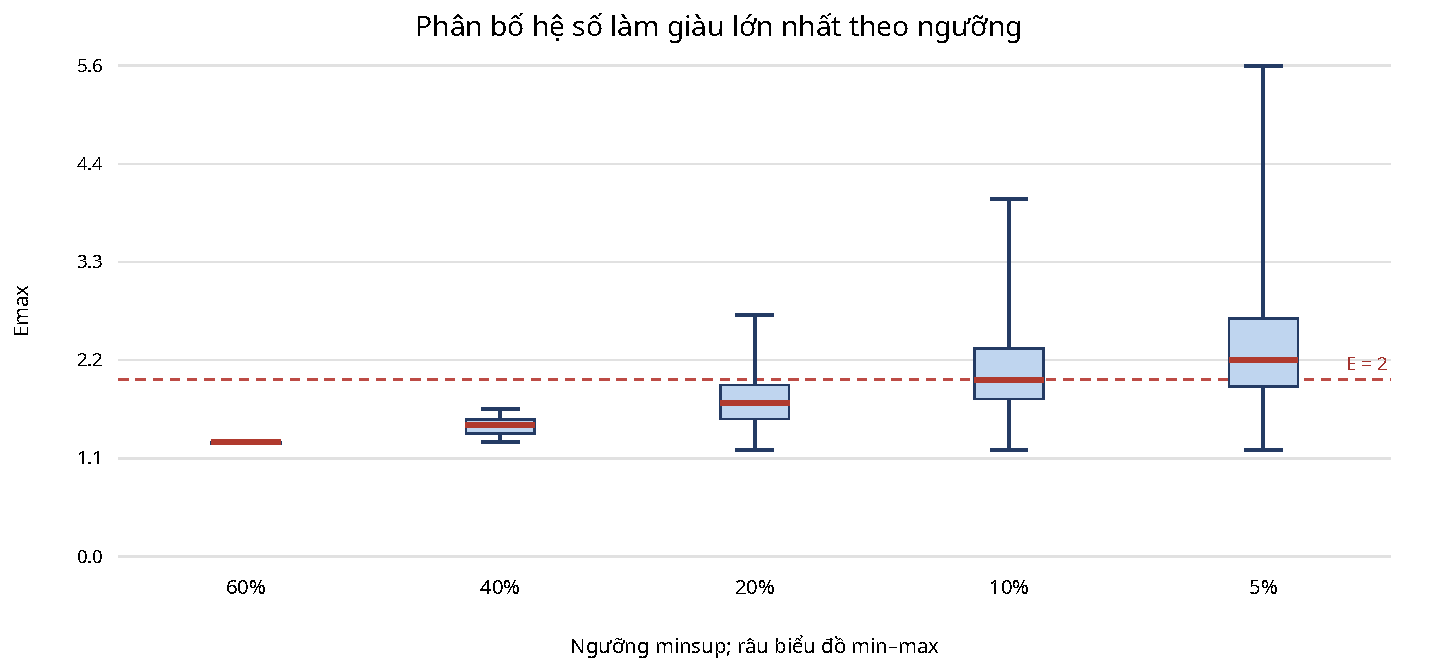
\includegraphics[width=\linewidth]{figures/notebook3/enrichment_by_threshold.pdf}
        \\
        \small (a) Phân bố $E_{\max}$ theo ngưỡng hỗ trợ.
    \end{minipage}\hfill
    \begin{minipage}[t]{0.48\textwidth}
        \centering
        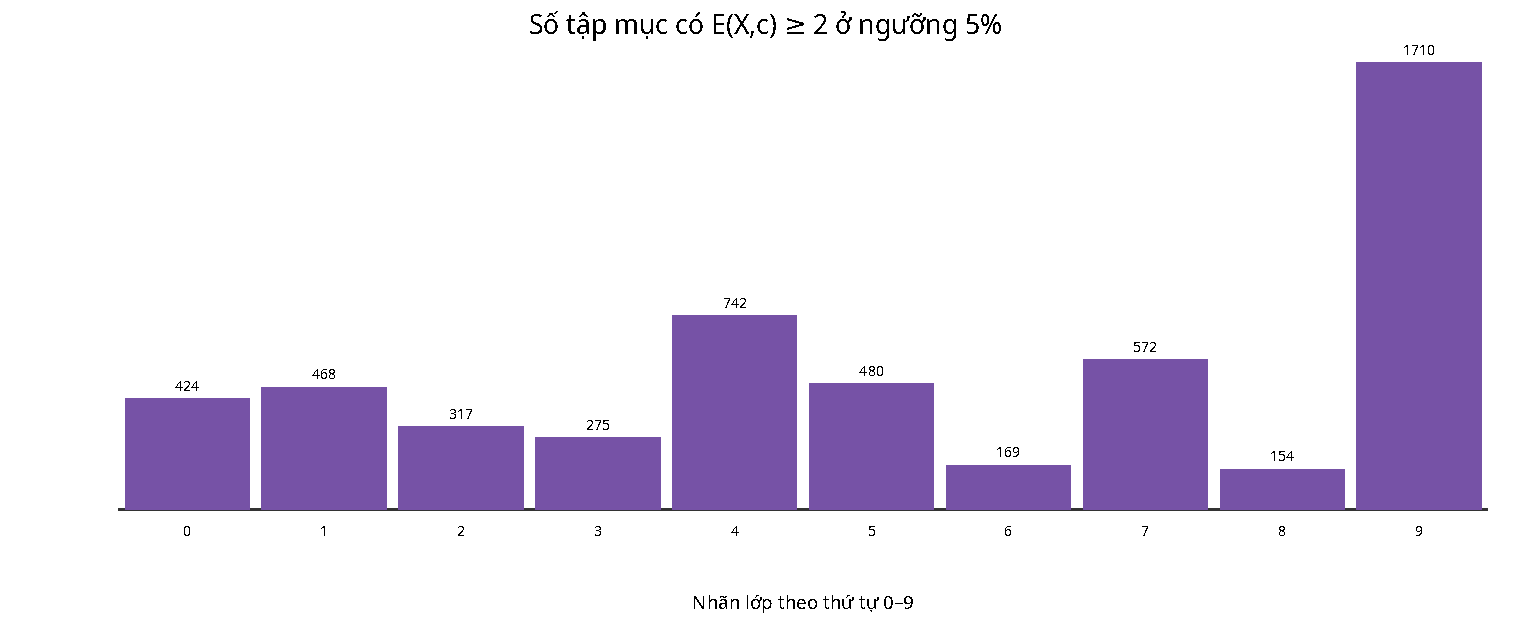
\includegraphics[width=\linewidth]{figures/notebook3/patterns_enriched_by_class.pdf}
        \\
        \small (b) Số tập mục có $E(X,c)\geq2$ theo lớp.
    \end{minipage}
    \caption{Mức độ làm giàu của các tập mục khai thác được. Râu ở biểu đồ (a) biểu thị khoảng giá trị nhỏ nhất–lớn nhất. Biểu đồ (b) đếm riêng theo từng lớp, nên một tập mục có thể xuất hiện trong nhiều cột.}
    \label{fig:fashion_enrichment_summary}
\end{figure*}

\subsection{Các mẫu nhiều mã nổi bật trong từng lớp}

Để xem tổ hợp từ thị giác nào gắn với từng lớp, nhóm chọn cho mỗi lớp một tập nhiều mã có $E(X,c)$ cao nhất trong số các tập mà ít nhất 10\% ảnh của lớp chứa tập đó. Hình~\ref{fig:fashion_class_pattern_heatmap} biểu diễn tỷ lệ chứa từng mẫu trên cả mười lớp. Ví dụ, mẫu $\{13,14,26,29\}$ có mặt trong 31,11\% ảnh Trouser và hệ số làm giàu 5,553; mẫu $\{3,10,15,22\}$ có mặt trong 25,91\% ảnh Ankle boot và hệ số 5,156. Các mẫu và số đo của mười lớp được liệt kê ở Phụ lục~\ref{app:fashion_enrichment}.

\begin{figure*}[!t]
    \centering
    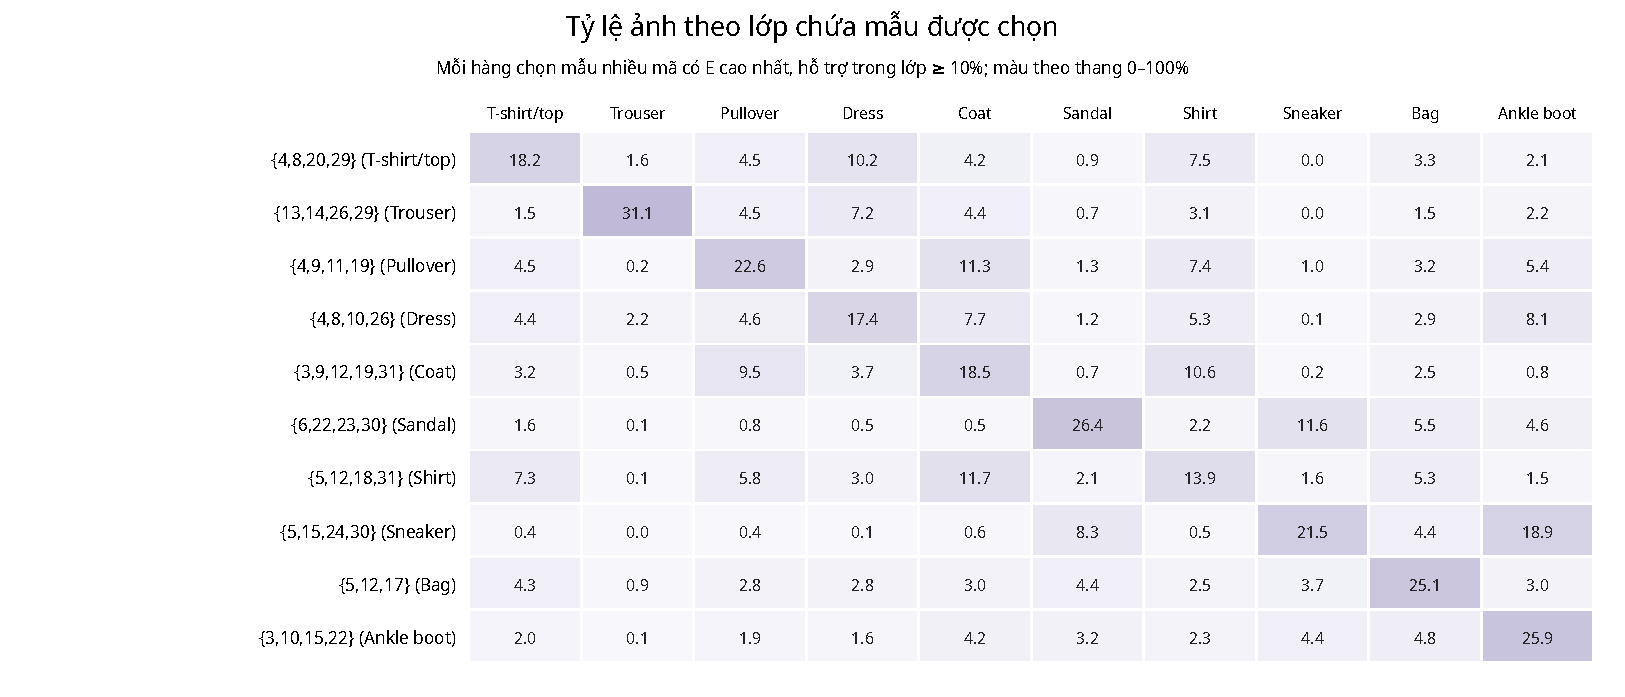
\includegraphics[width=0.98\textwidth]{figures/notebook3/class_pattern_heatmap.pdf}
    \caption{Tỷ lệ ảnh trong mỗi lớp chứa mẫu nhiều mã được chọn cho hàng đó. Mẫu của từng hàng được chọn theo hệ số làm giàu cao nhất, với điều kiện tỷ lệ hỗ trợ trong lớp đạt ít nhất 10\%.}
    \label{fig:fashion_class_pattern_heatmap}
\end{figure*}

Đây là các mẫu được sàng lọc và mô tả trên cùng 70.000 ảnh, không phải bộ luật dự đoán. Việc chọn mẫu theo hệ số lớn nhất trong mười lớp có thể làm nổi bật các chênh lệch ngẫu nhiên ở mẫu ít phổ biến; cần dữ liệu huấn luyện và kiểm thử tách biệt trước khi diễn giải chúng như tín hiệu phân loại.

\subsection{Hướng ứng dụng và phát triển các mô hình khác}

Các tập mục được làm giàu theo lớp có thể dùng làm đặc trưng dễ diễn giải cho bước phân loại tiếp theo. Chẳng hạn, mẫu $\{13,14,26,29\}$ xuất hiện trong 31,11\% ảnh Trouser và có hệ số làm giàu 5,553; mẫu $\{3,10,15,22\}$ xuất hiện trong 25,91\% ảnh Ankle boot và có hệ số 5,156. Các giá trị này giúp đề xuất những mẫu cần kiểm tra thêm, nhưng chưa chứng minh khả năng phân loại vì codebook và mẫu được khai thác từ cả 70.000 ảnh.

Với $m$ tập mục đã chọn $P_1,\ldots,P_m$, véc-tơ đặc trưng của ảnh $I_i$ là $\boldsymbol{\phi}(I_i)=(\phi_1(I_i),\ldots,\phi_m(I_i))$. Mỗi thành phần cho biết giao dịch $T_i$ có chứa tập mục tương ứng hay không:
\begin{equation}
    \phi_j(I_i)=\mathbf{1}\!\left[P_j\subseteq T_i\right],
    \qquad j=1,\ldots,m.
    \label{eq:fim_pattern_features}
\end{equation}
Véc-tơ này có thể được đánh giá cùng BoVW nhị phân 32 chiều bằng các mô hình như hồi quy logistic, SVM tuyến tính hoặc cây quyết định. Một hướng ứng dụng khác là tìm ảnh có chung các mẫu thị giác; khi đó các tập mục đóng vai trò mô tả để truy vấn và giải thích kết quả.

Để kiểm tra giá trị dự đoán, có thể dùng kiểm định chéo phân tầng 5 phần (stratified 5-fold cross-validation) trên 60.000 ảnh huấn luyện. Phân tầng giữ tỷ lệ lớp tương đối đồng đều giữa các phần. Ở mỗi vòng, bốn phần dùng để học codebook K-means, khai thác và chọn các tập mục $P_j$, xây dựng đặc trưng rồi huấn luyện mô hình; phần còn lại dùng để đánh giá vòng đó. Các bước học codebook, khai thác mẫu và chọn đặc trưng phải được làm lại chỉ trên bốn phần huấn luyện của vòng tương ứng. Nếu tính chúng trước trên toàn bộ dữ liệu rồi mới chia fold, ảnh validation đã ảnh hưởng đến đặc trưng và điểm đánh giá có thể lạc quan hơn thực tế.

Trên cùng các fold, nên so sánh ít nhất ba biểu diễn: BoVW nhị phân 32 chiều; véc-tơ chỉ báo cho biết ảnh có chứa từng tập mục đã chọn hay không; và biểu diễn có xét vị trí, trong đó mã thị giác được kết hợp với vùng hoặc tọa độ tương ứng. Với mỗi biểu diễn, có thể đánh giá cùng danh sách bộ phân loại như hồi quy logistic, SVM tuyến tính và cây quyết định. Các tham số cần khảo sát gồm số cụm $K$, ngưỡng hỗ trợ và độ dài tối đa của tập mục, độ phân giải biểu diễn không gian, cùng mức điều chuẩn hoặc độ sâu của mô hình. Việc chọn giá trị cho từng tổ hợp biểu diễn và mô hình chỉ dựa trên các fold huấn luyện và điểm validation tương ứng. Nên báo cáo trung bình và độ lệch chuẩn của độ chính xác và F1 vĩ mô qua năm fold; ma trận nhầm lẫn có thể tổng hợp từ các dự đoán ngoài fold để chỉ ra những lớp thường bị nhầm lẫn. Mọi biểu diễn và mô hình cần dùng cùng cách chia dữ liệu và cùng quy trình tìm kiếm tham số để so sánh công bằng.

Sau khi khóa biểu diễn, tham số và mô hình, huấn luyện lại pipeline đã chọn trên toàn bộ 60.000 ảnh huấn luyện rồi đánh giá đúng một lần trên 10.000 ảnh kiểm thử chưa tham gia học codebook, khai thác tập mục hay chọn tham số. Chỉ khi kết quả trên tập kiểm thử độc lập duy trì được mức cải thiện so với BoVW nhị phân cơ sở mới có cơ sở kết luận các tập mục hoặc thông tin vị trí đóng góp giá trị dự đoán.

\subsection{Kết luận}

Thí nghiệm minh họa cách biểu diễn ảnh Fashion-MNIST thành các giao dịch BoVW nhị phân để tìm những tổ hợp từ thị giác thường xuất hiện cùng nhau. Với 70.000 giao dịch, Eclat tìm được 6.185 tập mục ở minsup 5\%, và TID-set cùng BitVector cho kết quả trùng khớp hoàn toàn tại cả sáu ngưỡng đã khảo sát. Phân tích hậu nghiệm cho thấy một số mẫu được làm giàu ở từng lớp, nhưng mức độ phổ biến của chúng vẫn thay đổi giữa các lớp và có mẫu xuất hiện rộng khắp toàn bộ dữ liệu.

Các mẫu này có thể được dùng làm đặc trưng dễ diễn giải cho một mô hình phân loại hoặc công cụ truy vấn ảnh tương tự. Tuy vậy, đó mới là hướng ứng dụng cần kiểm chứng: dữ liệu kiểm thử đã tham gia học codebook và khai thác tập mục trong thí nghiệm hiện tại. Vì thế, kết quả chưa đo giá trị dự đoán. Cần xây dựng lại toàn bộ pipeline trong từng fold huấn luyện, so sánh các biểu diễn và mô hình bằng kiểm định chéo, rồi dùng tập kiểm thử riêng để xác nhận liệu các đặc trưng tập mục hoặc thông tin vị trí có tạo ra cải thiện hay không.

\begin{thebibliography}{99}
\bibitem{Sivic03}
J. Sivic and A. Zisserman,
``Video Google: A Text Retrieval Approach to Object Matching in Videos,''
in \textit{Proc. IEEE International Conference on Computer Vision (ICCV)},
vol. 2, pp. 1470--1477, 2003.

\bibitem{Hartigan1979}
J. A. Hartigan and M. A. Wong,
``Algorithm AS 136: A K-Means Clustering Algorithm,''
\textit{Journal of the Royal Statistical Society,
Series C (Applied Statistics)},
vol. 28, no. 1, pp. 100--108, 1979,
doi: 10.2307/2346830.

\bibitem{Zaki2000}
M. J. Zaki,
``Scalable Algorithms for Association Mining,''
\textit{IEEE Transactions on Knowledge and Data Engineering},
vol. 12, no. 3, pp. 372--390, 2000,
doi: 10.1109/69.846291.


\bibitem{Xiao2017}
H. Xiao, K. Rasul, and R. Vollgraf,
``Fashion-MNIST: A Novel Image Dataset for Benchmarking
Machine Learning Algorithms,''
\textit{arXiv preprint arXiv:1708.07747}, 2017,
doi: 10.48550/arXiv.1708.07747.


\end{thebibliography}

\clearpage
\appendices

\section{Khảo sát cấu hình và đặc điểm giao dịch}
\label{app:fashion_configuration}

\textit{Kích thước vùng ảnh.}
Lưới không chồng lấp trên ảnh $28\times28$ tạo 196, 49 hoặc 16 vùng khi cạnh vùng lần lượt là 2, 4 hoặc 7 pixel. Vùng nhỏ cho phép lọc nền chi tiết hơn nhưng làm tăng số vectơ cần xử lý. Vùng lớn chứa nhiều điểm ảnh lân cận hơn và có thể trộn nền với đường biên của vật thể. Trong phép đối chiếu $4\times4$ với $7\times7$, khi cả hai lưới loại khoảng 39,3\% số vùng, tỷ lệ gradient bị mất lần lượt là 5,92\% và 14,00\%. Kết quả là căn cứ thực nghiệm để dùng lưới $4\times4$.

\textit{Lọc nền.}
Quy tắc phát hành giữ một vùng nếu có ít nhất một pixel lớn hơn 29. Trên 70.000 ảnh, quy tắc này loại 37,50\% số vùng và làm mất 4,41\% tổng độ lớn gradient; mọi ảnh đều còn vùng. Tổng số descriptor dùng trong lượt K-means là 2.143.746 trên 3.430.000 vùng ban đầu.

\textit{Khảo sát số cụm.}
Bảng~\ref{tab:fashion_k_appendix} lưu kết quả khảo sát cấu hình trước khi tạo gói hiện tại. Các số này mô tả phép khảo sát $K$ đã lưu; số đo K-means của gói đang phân tích được trình bày riêng trong Bảng~\ref{tab:kmeans_configuration}.

\begin{center}
    \captionof{table}{Kết quả khảo sát cấu hình K-means}
    \label{tab:fashion_k_appendix}
    \footnotesize
    \begin{tabular}{@{}rrrr@{}}
        \toprule
        $K$ & Độ méo & Số mã trung bình/giao dịch & Hội tụ \\
        \midrule
        16  & 0,441 &  9,00 & Có \\
        32  & 0,347 & 12,27 & Có \\
        64  & 0,271 & 15,11 & Có \\
        128 & 0,219 & 17,99 & Có \\
        256 & 0,177 & 20,29 & Chưa \\
        \bottomrule
    \end{tabular}
\end{center}

Khảo sát cho thấy khi tăng $K$, độ méo giảm nhưng số mã trung bình
trong mỗi giao dịch tăng. Nhóm giữ $K=32$ làm cấu hình cho lượt phân
tích tiếp theo; bảng này không chứng minh $K=32$ tối ưu theo mọi tiêu chí.

\textit{Thống kê giao dịch của gói hiện tại.}
Sau khi gộp các mã lặp trong từng ảnh, 70.000 giao dịch có 856.373 lượt xuất hiện của 32 mã. Độ dài giao dịch từ 2 đến 24; trung bình 12,2339, trung vị 12 và độ lệch chuẩn tổng thể 3,0061. Mật độ là $856\,373/(70\,000\times32)=38,23\%$. Không có giao dịch rỗng.

Tham khảo \href{https://github.com/NguyenVoTanDuy2006/DataMining-FIM-Project/blob/dbadabc4af05070c602b3bcd890150fcd496c885/docs/UD2/TC_plan.md}{khảo sát tiền xử lý ảnh} và \href{https://github.com/NguyenVoTanDuy2006/DataMining-FIM-Project/blob/dbadabc4af05070c602b3bcd890150fcd496c885/notebooks/fashion-mnist/demo/01_image_exploration.ipynb}{phần khảo sát ảnh}.

\newpage
\section{Đối chiếu kết quả khai thác}
\label{app:fashion_eclat}

\textit{Độ hỗ trợ trên BoVW nhị phân.}
Gọi $D(w)$ là tập giao dịch chứa từ thị giác $w$ và $N$ là số giao dịch. Độ hỗ trợ của tập mục $X$ là
\[
    \operatorname{supp}(X)
    = \frac{\left|\bigcap_{w\in X} D(w)\right|}{N}.
\]
Chẳng hạn, với ba giao dịch $\{1,6\}$, $\{6,24\}$ và $\{1,6,24\}$, tập $\{1,6\}$ có độ hỗ trợ $2/3$.

\textit{Đối chiếu hai backend.}
Bảng~\ref{tab:fashion_audit_appendix} ghi số tập mục trả về trên cùng bộ giao dịch và kết quả so sánh đầy đủ từng tập cùng số hỗ trợ. Hai backend cho kết quả giống nhau ở cả sáu ngưỡng.

\begin{center}
    \captionof{table}{Số tập mục phổ biến và kết quả so sánh Set với BitVector}
    \label{tab:fashion_audit_appendix}
    \footnotesize
    \setlength{\tabcolsep}{4pt}
    \begin{tabular}{@{}crrrc@{}}
        \toprule
        Ngưỡng & Số hỗ trợ tối thiểu & Set & BitVector & Giống nhau \\
        \midrule
        80\% & 56.000 & 0 & 0 & PASS \\
        60\% & 42.000 & 1 & 1 & PASS \\
        40\% & 28.000 & 11 & 11 & PASS \\
        20\% & 14.000 & 145 & 145 & PASS \\
        10\% & 7.000 & 1.098 & 1.098 & PASS \\
         5\% & 3.500 & 6.185 & 6.185 & PASS \\
        \bottomrule
    \end{tabular}
\end{center}

Tại ngưỡng 5\%, phân bố độ dài tập mục là:

\begin{center}
    \captionof{table}{Số tập mục theo độ dài ở ngưỡng 5\%}
    \label{tab:fashion_itemset_lengths}
    \footnotesize
    \begin{tabular}{@{}rr@{}}
        \toprule
        Độ dài & Số tập mục \\
        \midrule
        1 & 32 \\
        2 & 482 \\
        3 & 2.468 \\
        4 & 2.681 \\
        5 & 508 \\
        6 & 14 \\
        \bottomrule
    \end{tabular}
\end{center}

\textit{Thời gian Eclat.}
Bảng~\ref{tab:fashion_eclat_measurements} ghi số đo trong tiến trình riêng cho sáu ngưỡng. Tỷ số được tính bằng thời gian Set chia cho thời gian BitVector; giá trị lớn hơn 1 nghĩa là BitVector nhanh hơn trong lượt đo đó.

\begin{center}
    \captionof{table}{Thời gian Eclat theo cách cài đặt và ngưỡng hỗ trợ}
    \label{tab:fashion_eclat_measurements}
    \scriptsize
    \setlength{\tabcolsep}{4pt}
    \begin{tabular}{@{}c r r r@{}}
        \toprule
        Ngưỡng & Set (s) & BitVector (s) & Tỷ số Set/BitVector \\
        \midrule
        80\% & 4,580 & 4,161 & 1,10$\times$ \\
        60\% & 4,755 & 4,493 & 1,06$\times$ \\
        40\% & 5,260 & 5,380 & 0,98$\times$ \\
        20\% & 7,629 & 6,097 & 1,25$\times$ \\
        10\% & 11,862 & 7,467 & 1,59$\times$ \\
         5\% & 20,937 & 8,727 & 2,40$\times$ \\
        \bottomrule
    \end{tabular}
\end{center}

Mỗi cấu hình được đo một lượt, không có lượt làm nóng và không đo lặp; do đó bảng không đủ để kết luận chênh lệch thời gian có ổn định giữa các lần chạy hay môi trường hay không. Thời gian tiến trình đo tính từ lúc đọc tệp giao dịch đến khi ghi kết quả.

\newpage
\section{Phân tích mẫu theo lớp}
\label{app:fashion_enrichment}

\textit{Các mẫu đại diện ở ngưỡng 5\%.}
Bảng~\ref{tab:fashion_representative_patterns} ghi bốn mẫu được chọn theo quy tắc phân tích đã áp dụng: mẫu đơn hỗ trợ cao nhất, cặp hỗ trợ cao nhất, tập từ ba mã trở lên hỗ trợ cao nhất và một mẫu nhiều mã có hỗ trợ dưới 10\%. Mẫu cuối có mức làm giàu cao nhất trong bốn ví dụ, nhưng vẫn là mô tả hậu nghiệm trên toàn bộ dữ liệu.

\begin{center}
    \captionof{table}{Bốn mẫu đại diện được truy vết}
    \label{tab:fashion_representative_patterns}
    \scriptsize
    \setlength{\tabcolsep}{2pt}
    \begin{tabular}{@{}l r r l r@{}}
        \toprule
        Mẫu & Hỗ trợ & Toàn cục (\%) & \shortstack{Lớp $E$ cao nhất\\Tỷ lệ trong lớp (\%)} & $E_{\max}$ \\
        \midrule
        $\{6\}$ & 49.181 & 70,259 & Sandal (90,94) & 1,294 \\
        $\{6,12\}$ & 29.223 & 41,747 & T-shirt/top (62,20) & 1,490 \\
        $\{6,12,22\}$ & 16.218 & 23,169 & Sandal (37,30) & 1,610 \\
        $\{6,15,17\}$ & 6.991 & 9,987 & Sandal (31,17) & 3,121 \\
        \bottomrule
    \end{tabular}
\end{center}

\textit{Số tập được làm giàu theo lớp.}
Ở ngưỡng hỗ trợ 5\%, số tập mục có $E(X,c)\geq2$ theo lớp lần lượt là:

\begin{center}
    \captionof{table}{Số tập mục có hệ số làm giàu ít nhất 2 theo lớp}
    \label{tab:fashion_enriched_counts_by_class}
    \scriptsize
    \begin{tabular}{@{}l r@{\qquad}l r@{}}
        \toprule
        Lớp & Số tập mục & Lớp & Số tập mục \\
        \midrule
        T-shirt/top & 424 & Trouser & 468 \\
        Pullover & 317 & Dress & 275 \\
        Coat & 742 & Sandal & 480 \\
        Shirt & 169 & Sneaker & 572 \\
        Bag & 154 & Ankle boot & 1.710 \\
        \bottomrule
    \end{tabular}
\end{center}

Các số đếm không loại trừ nhau vì cùng một tập mục có thể được làm giàu trong nhiều lớp. Ankle boot có số tập đạt ngưỡng nhiều nhất (1.710), nhưng con số này không đồng nghĩa với độ chính xác phân loại hay khả năng nhận diện lớp.

\textit{Một mẫu nhiều mã cho mỗi lớp.}
Bảng~\ref{tab:fashion_top_pattern_per_class} liệt kê các hàng trong Hình~\ref{fig:fashion_class_pattern_heatmap}. Mỗi mẫu được chọn trong nhóm có ít nhất 10\% ảnh của lớp đích hỗ trợ; cột tỷ lệ trong lớp là $P(X\mid c)$.

\begin{center}
    \captionof{table}{Mẫu có hệ số làm giàu cao nhất trong từng lớp}
    \label{tab:fashion_top_pattern_per_class}
    \scriptsize
    \setlength{\tabcolsep}{2pt}
    \begin{tabular}{@{}l l r r r@{}}
        \toprule
        Lớp đích & Mẫu & Số ảnh hỗ trợ & Tỷ lệ trong lớp (\%) & $E(X,c)$ \\
        \midrule
        T-shirt/top & $\{4,8,20,29\}$ & 3.665 & 18,20 & 3,476 \\
        Trouser & $\{13,14,26,29\}$ & 3.922 & 31,11 & 5,553 \\
        Pullover & $\{4,9,11,19\}$ & 4.174 & 22,56 & 3,783 \\
        Dress & $\{4,8,10,26\}$ & 3.780 & 17,36 & 3,214 \\
        Coat & $\{3,9,12,19,31\}$ & 3.511 & 18,54 & 3,697 \\
        Sandal & $\{6,22,23,30\}$ & 3.759 & 26,37 & 4,911 \\
        Shirt & $\{5,12,18,31\}$ & 3.659 & 13,89 & 2,656 \\
        Sneaker & $\{5,15,24,30\}$ & 3.849 & 21,46 & 3,902 \\
        Bag & $\{5,12,17\}$ & 3.674 & 25,11 & 4,785 \\
        Ankle boot & $\{3,10,15,22\}$ & 3.518 & 25,91 & 5,156 \\
        \bottomrule
    \end{tabular}
\end{center}

Các tỷ lệ này mô tả đồng xuất hiện của từ thị giác trong ảnh thuộc mỗi lớp. Nhãn lớp được dùng sau khai thác; do codebook và tập mục đều được tạo từ cả tập huấn luyện lẫn kiểm thử, không xem các con số là đánh giá độc lập. Xem \href{https://github.com/NguyenVoTanDuy2006/DataMining-FIM-Project/blob/dbadabc4af05070c602b3bcd890150fcd496c885/notebooks/fashion-mnist/demo/03_transaction_exploration_and_mining.ipynb}{tài liệu phân tích giao dịch trên GitHub} để biết quy tắc chọn, kiểm tra đối chiếu và truy vết.

\end{document}
